\chapter{Критерии идентификации}

\section{Свойства и параметры критериев идентификации} % {{{1

Особенность динамики хаотических систем не позволяет
определить цель идентификации как задачу минимизации
какой-либо меры $\mu(x_o(t),x_i(t))$ в пространстве выходных
сигналов~[].

\Cmt{TODO: обоснование и картинки}

На рис.~\ref{atu:f:lor_diff_x0} приведён пример, показывающий
различие траекторий для системы Лоренца \Cmt{ref}
при малом возмущении значений начальных условий.

\begin{figure}[h!]
  \centerline{
    \includegraphics[width=0.49\textwidth]{p/lor_diff-p_xx_x0.png}
    \hfill
    \includegraphics[width=0.49\textwidth]{p/lor_diff-p_dx_x0.png}
  }
  \caption{Различине в поведение системы Лоренца при малом возмущении начальных условий}
  \label{atu:f:lor_diff_x0}
\end{figure}


На рис.~\ref{atu:f:lor_diff_sigma} приведён пример, показвающий
различие траекторий для системы Лоренца
при малом возмущении значений параметра $\sigma$.

\begin{figure}[h!]
  \centerline{
    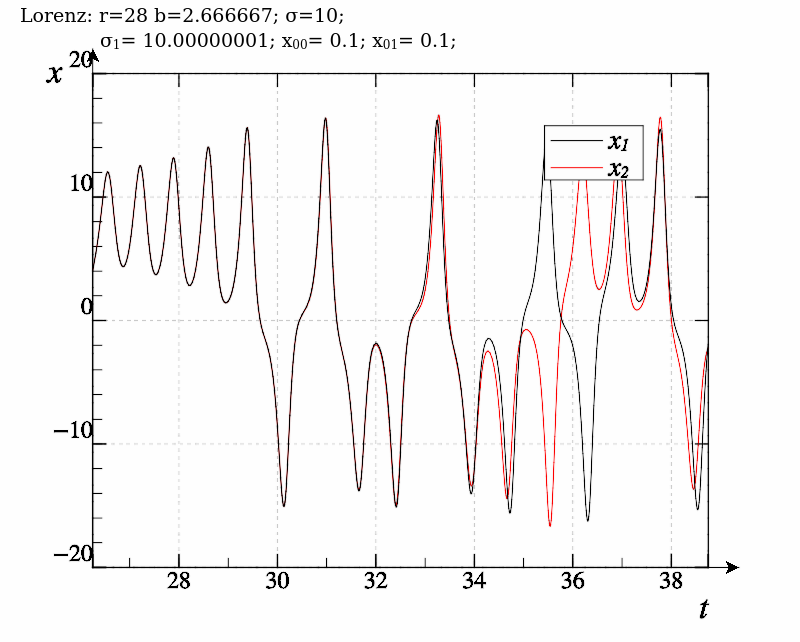
\includegraphics[width=0.49\textwidth]{p/lor_diff-p_xx_sigma.png}
    \hfill
    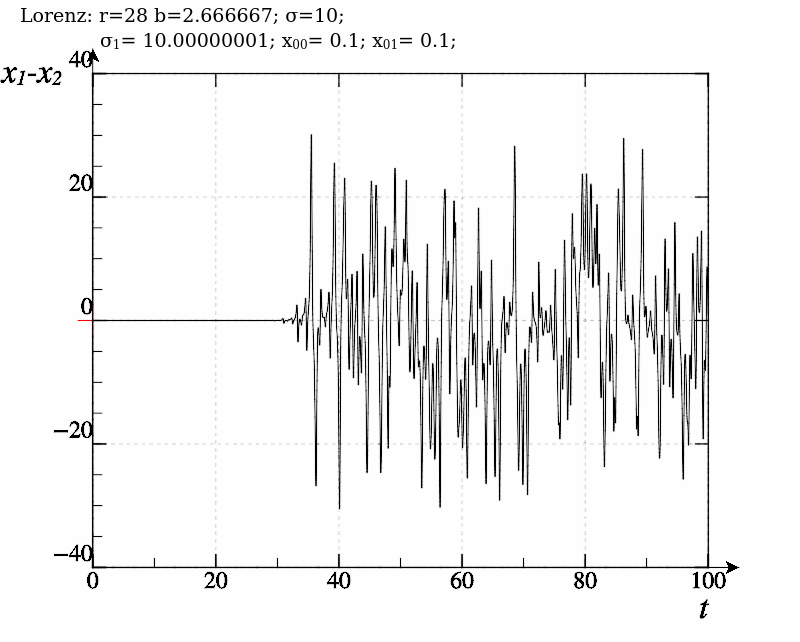
\includegraphics[width=0.49\textwidth]{p/lor_diff-p_dx_sigma.png}
  }
  \caption{Различине в поведение системы Лоренца при малом возмущении параметра $\sigma$}
  \label{atu:f:lor_diff_sigma}
\end{figure}


Для целей идентификации необходимо существование
заданного скалярного критерия $q(x(t))$, близость величин
которых для объекта и модели (в смысле какой-либо меры)
и позволяет говорить о достижении цели идентификации.

Для создания возможности использования критерия
для целей идентификации динамических системы,
сам критерий должен каким-либо образом отображать
глобальные свойства системы, а не её состояния в конкретный момент времени,
то есть не изменяться (по крайней мере существенно),
если свойства системы, предъявляемые в математичкой модели параметрами,
не изменяются. В таких случаях имеет смысл использовать
термин ``интегральные критерии''.



Существует множество способов определения критериев~[XXX].
Для достаточно простых систем вид критерия,
подходящего для задачи идентификации, можно вывести
определив каким-либо образом исходя из структуры
математической модели.
В некоторых случаях случаях вид критерия можно подобрать эмпирически,
на основании опыта в синтезе систем идентификации для подобных
систем. Тем не менее, наиболее обоснованным
является подход, основанный на использовании
каких-либо физических инвариантов.

Практически в каждом разделе физики существуют
определённые законы сохранения.
Прежде всего стоит назвать общеизвестные и всеобщие
законы сохранения энергии, импульса, момента импульса.
Также существуют и применяются законы сохранения
электрического, лептонного и барионного зарядов,
принцип бесцветности и т.д.

Наиболее общим, и, следовательно, наиболее употребляемым является
закон сохранения энергии.
Помимо закона сохранения энергии, существуют области,
где имеет смысл применять другие, вплоть до синтетических
законов сохранения, но этот подход
применяется реже.

Каждый из законов сохранения является инвариантом,
и может служить для синтеза критерия в какой-либо области
при определённых условиях.
Тем не менее, непосредственно применение
физических законов сохранения не всегда
удобно и прямолинейно.
Например, в теории управления системы динамического
хаоса относят к ``диссипативным'' системам.
Сам этот термин несколько отличается от аналогичного,
применяемого в физике.
Там система считается диссипативной, если она не
получает энергию извне, а имеющуюся переводит
в не описываемую рассматриваемым комплексом взаимодействий
форму, чаще всего в тепло. \Cmt{ref}
В теории управления
считается, что система, сохраняя процесс диссипации
(перевода энергии в неконтролируемую форму),
получает энергию извне, что и обеспечивает её незатухающую
динамику. \Cmt{ref}
Более того, сам вид уже существующих
математических моделей хаотических систем не позволяет
явно выделить понятие энергии в чистом виде.
В таких случаях
приходится прибегать к полуэмпирическим методам,
рассматривая доступные переменные состояния системы,
проводя анализ их влияния и, в результате моделирования,
выбирая подходящий вид критерия.

\Cmt{ Слова о том, что ``ы среднем''}


Рассмотрим основные способы представления энергии:

Кинетическая энергия тела массой $m$, которое движется со скоростью $v$:
%
\begin{equation}
  E_k = \frac{mv^2}{2} = \frac{m}{2} \left( \od{x}{t} \right)^2.
  \label{atu:eq:Ek_v}
\end{equation}
%
Следует обратить внимание, что, по сравнению с классическим
представлением энергии при обработке сигналов,
здесь присутствует квадратичная зависимость от производной сигнала.

Потенциальная энергия в однородном поле (нулевой уровень выбирается произвольно):
%
\begin{equation}
  E_p = m g x .
  \label{atu:eq:Ep_g}
\end{equation}

Потенциальная энергия в упругом приближении:
%
\begin{equation}
  E_p = k \frac{x^2}{2} .
  \label{atu:eq:Ep_spring}
\end{equation}

Кинетическая энергия вращающегося тела:
%
\begin{equation}
  E_k = J \frac{\omega^2}{2} = \frac{J}{2} \left( \od{\varphi}{t} \right)^2 .
  \label{atu:eq:Ek_spin}
\end{equation}

Внутренняя тепловая энергия:
%
\begin{equation}
  E_t = \frac{im}{2M} RT.
  \label{atu:eq:Et}
\end{equation}

Электрическая энергия, накопленная в конденсаторе:
%
\begin{equation}
  E_c = \frac{C U^2}{2}.
  \label{atu:eq:Ec}
\end{equation}

Энергия магнитного поля, накопленная в катушке индуктивности:
%
\begin{equation}
  E_l = \frac{L I^2}{2} = \frac{L}{2} \left( \od{Q}{t}\right)^2 .
  \label{atu:eq:El}
\end{equation}

Энергия, превращаемая в тепло омическим сопротивлением:
%
\begin{equation}
  E_r = U I = I^2 R = \frac{U^2}{R} = U \od{Q}{t} .
  \label{atu:eq:Er}
\end{equation}



\Cmt{Chemical kinetic -- $\max(x)$}.

\Cmt{Electro-magnetic -- $x\cdot y$}.


Обобщая вышеизложенное, можно сделать выводы, что
несмотря на разнообразие физических процессов, количество способов
представления энергии (рассматриваем сосредоточенные параметры)
весьма ограничено. Основные виды зависимостей:

\begin{itemize}

  \item
    Квадратичная зависимость от координаты: $E \sim x^2$.

  \item
    Линейная зависимость от координаты: $E \sim x$.

  \item
    Квадратичная зависимость от производной координаты по времени: $E \sim \left( \od{x}{t}\right)^2$.

  \item
    Линейная зависимость от произведений координат: $E \sim x \cdot y$.

  \item
    Линейная зависимость от произведений одной координаты на производную другой: $E \sim x \cdot \od{y}{t}$.

\end{itemize}




Физическая измеримость.

Следствием невозможности непосредственного использования выходных
сигналов объекта и моделей в качестве критерия идентификации, а также
требование физической измеримости критерия является
тот факт, что для получения оценки критерия, как правило,
требуется значительное время.






Монотонность -- как следствие одноэкстремальность?


Зависимость (обозначение?) от времени оценивания.
Методы измерения.



% }}}1


\section{Отличие задачи идентификации от задач решения нелинейного уравнения и поиска экстремума} % {{{1

\Cmt{Перенести куда-то}

На первый взгляд, при заданном критерии идентификации, задача идентификации
сводится к классической задаче решения нелинейного уравнения: надо найти такие значения
параметров $p$, при которых критерий модели (или какой-либо из моделей)
$q_m$ принимает значение, наиболее близкое к значению критерия объекта $q_o$:
\[
  \mu( q_o, q_m(p) ) \to \min.
\]
Или же при использовании функции качества идентификации $F(q_o, q_m )$ задача
эквивалентна классической задаче поиска экстремума:
\[
  F( q_o, q_m(p) ) \to \max.
\]
На самом деле, существуют определённые аспекты, которые делают такое
сведение практически невозможным.

Прежде всего, в задаче в обеих исходных задачах
предполагается, что наблюдаемая система статична:
значение критерия не зависит от времени, и проведя измерение
в точке один раз, можно к нему не возвращаться.
Напротив, идентификация динамической системы предполагает,
что значение критерия, даже после какого-либо усреднения на конечном
интервале времени, есть величина динамическая, причём динамика определяется
не только параметрами системы, но и свойствами самой системы измерения,
а также процессом взаимодействия системы измерения с моделями. При этом
возможны весьма нетривиальные явления, такие как параметрический
резонанс, распространение параметрических волн на множестве моделей и т.д.

Также существенную роль могут играть как шумы измерения, так и побочные
эффекты от процесса фильтрации шумов.
Применение практически любого фильтра приводит к запаздыванию
в процессе измерения, и игнорирование этих явлений может привести
как к нарушению устойчивости поиска, так и получению совершенно
неадекватных результатов при наличии устойчивости.

В исходных задачах предполагается, что не только
значение функции известно точно в каждой точке, но также известны все производные
(по крайней мере, необходимые для работы метода).
В реальные задачах идентификации производные непосредственно
не доступны для измерения, а их оценка требует применения специальных
методов. При этом процесс оценивания производных, как правило,
более чувствителен к шумам измерения, чем собственно измерение.


\Cmt{ TODO: Требование конечности производных в условиях дискретного представления сигнала.}

Все эти явления делают задачу идентификации более сложной, чем
исходные задачи, чем и обусловлено
существование широкого спектра методов идентификации. Тем не менее,
некоторые алгоритмы, применимые при поиска экстремума, могут быть
полезны при синтезе системы идентификации.

Свёртка с чем-то.

Как уже было отмечено, для успешности процесса идентификации требуется
построение различных интегральных критериев, зависящих,
хотя бы в первом приближении
от величины идентифицируемого параметра. Конкретный вид определяется самим идентифицируемым
объектом. При этом, довольно часто (но не всегда) в качестве основы для такого критерия выступает
некая энергетическая зависимость. С учётом усреднения на требуемом интервале,
один из простых видов критерия может быть задан как
%
\begin{equation}
\od{q_{x^2}}{t}
=
\frac{1}{\tau_q} \left( x^2(t) - q_{x^2}(t) \right)
,
\label{atu:eq:qlin}
\end{equation}
%
%\noindent
где $\tau_q$ -- характерное время оценивания, $x(t)$ -- выбранная переменная состояния системы.

Скользящее среднее:
$q_{ma}$??

Чернавскиий~\cite{chernavskii_syn_info}.

% }}}1

\section{Выводы по разделу \thechapter}  % {{{1

Выводы.

% }}}1

% vim: fdm=marker ft=tex
